\section{How does sampling work?}
\label{sec:hws_how}

While the last section was concerned with \textit{what} the hws library can sample, this section explains \textit{how} it is implemented. 



The general flow of the hws library looks as follows:
\begin{enumerate}
    \item%
    A new hardware sampler is constructed, initializing the required environment from the respective vendor library. 
    An atomic reference count is used to ensure that the respective environments are only initialized once. 
    Note that it is supported to start as many hardware samplers as one wishes and that combination of different hardware samplers is supported. 
    If everything should be sampled, it is easiest to use a \code{system_hardware_sampler}.
    \item%
    A hardware sampler is then started using the \code{start_sampling()} function which internally spawns a new \code{std::thread}. 
    The actual sampling process then takes place asynchronously in this newly created thread. 
    Note that one thread is created for each hardware sampler. 
    The \code{system_hardware_sampler} also starts as many threads as it encapsulates other hardware samplers. 
    \item%
    All supported hardware samples are initialized: The fixed samples to their final values and the running samples to their first value. 
    This step is also used to determine which hardware samples are supported on the current hardware. 
    All theoretically by hws supported samples are queried and if the respective vendor function returns with an error, i.e., a sample is not supported, the value will be set to an \code{std::nullopt} indicating that it can be ignored in future sampling attempts during the sampling loop. 
    \item%
    The actual sampling loop is started. 
    Here, a new value is added to every supported running sample. 
    At the end, the current thread sleeps for the amount of time specified by the sampling interval before it starts again to sample new values. 
    Using the \code{pause_sampling()} and \code{resume_sampling()} functions, the sampling of new values can temporarily be paused using an atomic flag as a signaling variable. 
    \item%
    At the end, one must call the \code{stop_sampling()} function which waits until the current sampling loop has finished and then joins on the previously spawned \code{std::thread}. 
    Note that once a hardware sampler has been stopped, it cannot be started again. 
    \item%
    Only after the hardware sampler has been stopped, all samples can be saved to a YAML file using the \code{dump_yaml(filename)} function. 
    Note that it is still possible to retrieve the current hardware samples programmatically during the program execution.
    \item%
    At the end of the lifetime of a hardware sampler, in its constructor the previously mentioned reference count is decreased and only if it reaches zero, the respective vendor specific environment is shut down ensuring this only happens once. 
\end{enumerate}

\subsection{Hardware Sampling Implementation}

I have to differentiate the hws internal implementation targeting \glspl{cpu} and \glspl{gpu}.
To sample information on the supported \glspl{gpu}, I use the respective vendor-provided library. 
For NVIDIA \glspl{gpu} this is the \gls{nvml} library, for AMD \glspl{gpu} it is the \gls{rocmsmi} library, and for Intel \glspl{gpu} it is the Level Zero library. 
While the \glspl{api} are relatively similar for \gls{nvml} and \gls{rocmsmi}, Level Zero has a significantly different approach, which can also be seen in \autoref{code:vendor_library_calls}. 
Nevertheless, all functions are simple library calls.

On the \gls{cpu}, however, this is different since there is no simple library that I can call to gather all the necessary information. 
Here, I use three different command line utilities: to retrieve general \gls{cpu} information, like core-count, socket-count, cache-sizes, etc., I use \texttt{lscpu}~\cite{qian_lscpu_nodate}, for memory-related information, i.e., available, used, and total main memory, I use \texttt{free}~\cite{small_free_nodate}, and for everything else like frequency or power related information I use \texttt{turbostat}~\cite{brown_turbostat_nodate}. 
In all three cases, I create a new subprocess, call the respective utility, and then return the standard output as a string. 
This string contains all necessary information and is then post-processed to extract the data inside the \gls{cpu} hardware sampler. 
For \texttt{lscpu}, the subprocess simply calls \texttt{lscpu}. 
In the case of the \texttt{free} command, the command line flag \texttt{-b} is added to be sure that the memory size information is output in bytes. 
For \texttt{turbostat} it is a bit different. 
First, I have to note that to get the full \texttt{turbostat} information, it has to be called with root privileges. 
However, in newer \texttt{turbostat} versions, it is possible to get a subset of all possible information even if \texttt{turbostat} is not called with root privileges. 
I handle that distinction directly in CMake: it tests whether \texttt{turbostat} can be executed with root privileges and if this is not the case it tests whether it can be executed without root privileges. 
In the latter case, gathering information via \texttt{turbostat} is completely disabled. 
In the former case, I sample the information using the \texttt{turbostat} command \texttt{sudo turbostat -n 1 -i 0.001 -S -q} with \texttt{sudo} only present if \texttt{turbostat} can be executed with root privileges. 
This command samples all available information immediately (\texttt{-i 0.001}) exactly once (\texttt{-n 1}) and outputs the information in a short summary format (\texttt{-S}) skipping potential header information (\texttt{-q}). 
An example \texttt{turbostat} output with the mentioned command looks like displayed in \autoref{code:turbostat_output}. 

\begin{listing}
    \begin{moderncode}[fontsize=\setfontsize{6.5}]{text}
Avg_MHz  Busy%  Bzy_MHz  TSC_MHz  IPC   IRQ  POLL  C1   C2   POLL%  C1%   C2%     CorWatt  PkgWatt
39       1.77   2212     4686     0.92  818  1     156  819  0.01   3.03  110.73  4.58     264.06
    \end{moderncode}
    \caption{%
    An example output of the command \texttt{sudo turbostat -n 1 -i 0.001 -S -q} with root privileges enabled for \texttt{turbostat} on an AMD EPYC 9274F \gls{cpu}.
    }
    \label{code:turbostat_output}
\end{listing}
Note that the output of \texttt{turbostat} also depends on the used \gls{cpu}. 
For example, the output \autoref{code:turbostat_output} was gathered on an AMD EPYC 9274F \gls{cpu} and consists of $14$ table entries. 
If I run the same command for example on an Intel i5-10210U \gls{cpu}, the output consists of $52$ columns mostly adding more idle state information but also temperature-related information missing for the AMD \gls{cpu}.

\todo{remake plot (new runtimes with more data points)}
\begin{figure}
    \centering
    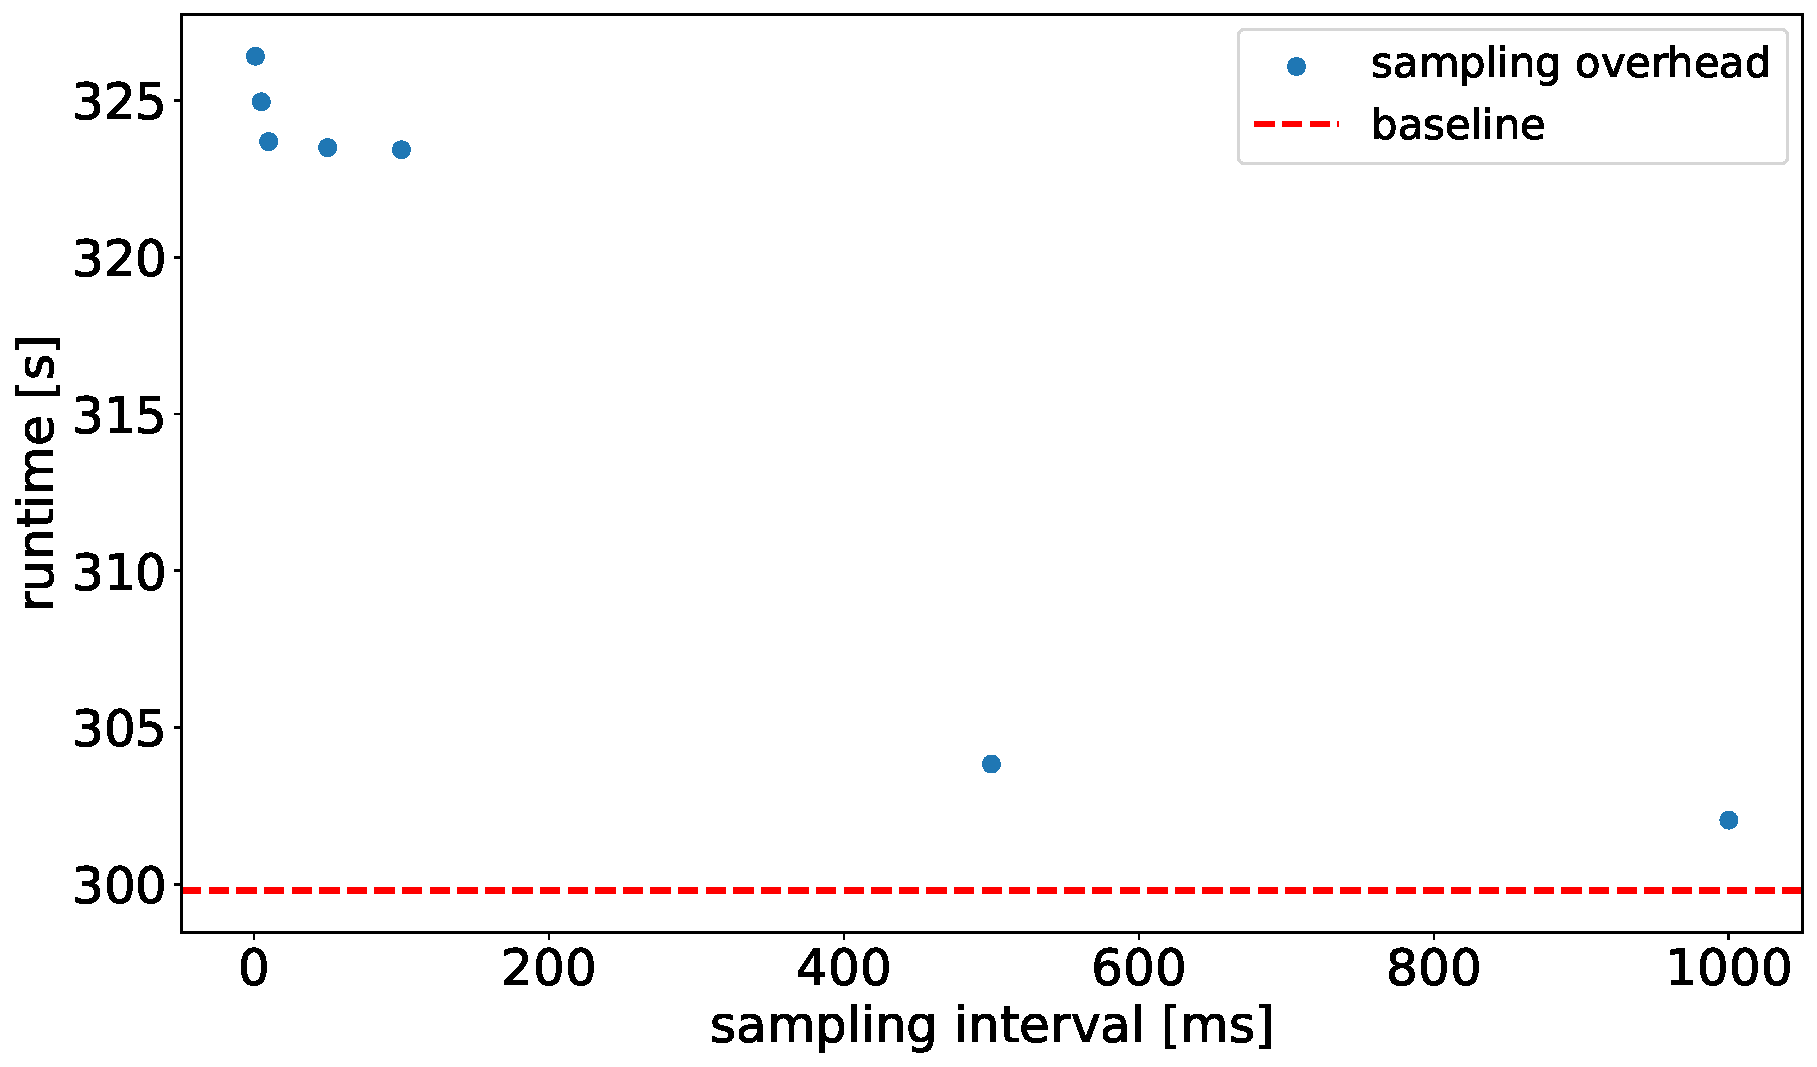
\includegraphics[width=0.8\linewidth]{figures/03_performance_sampling_hws/hws_sampling_interval_overhead.pdf}
    \caption{%
    The overhead when using the hws library, depends on the specified sampling interval. 
    The red dashed line at the bottom is the baseline version without hws. 
    We can see, that the overhead when using hws is noticeable for smaller sampling intervals. 
    However, increasing the sampling interval also drastically decreases the overhead. 
    }
    \label{fig:hws_overhead}
\end{figure}